
\documentclass[tikz,border=5pt]{standalone}

% Core packages
\usepackage{amsmath,amssymb}
\usepackage{tikz}
\usepackage{tikz-cd}
\usepackage{pgfplots}
\usepackage{multicol}
\usepackage{xcolor}
\usepackage{caption}
\usepackage{float}
\usepackage{kotex}

% TikZ / PGF configuration
\usetikzlibrary{
  arrows.meta,
  calc,
  positioning,
  shapes.geometric,
  shapes.symbols,
  fit,
  backgrounds,
  patterns,
  matrix,
  intersections,
  decorations.pathmorphing,
  decorations.markings,
  angles,
  quotes
}
\pgfplotsset{compat=1.18}

% Reusable TikZ styles
\tikzset{
  >=stealth,
  line cap=round,
  line join=round,
  every picture/.style={line width=0.9pt},
  box/.style={draw, rounded corners, minimum width=2.8cm, minimum height=1.2cm, align=center},
  circlebox/.style={draw, circle, minimum size=1cm, align=center},
  arrow/.style={->, thick},
  dashedarrow/.style={->, thick, dashed},
  point/.style={circle, fill, inner sep=1.2pt},
  gridhelp/.style={help lines, gray!35},
  highlight/.style={fill=blue!10, draw=blue!60!black},
  3D/.style={
    x={(-0.60cm,-0.42cm)},
    y={(0.78cm,0cm)},
    z={(0cm,0.78cm)}
  }
}


\begin{document}

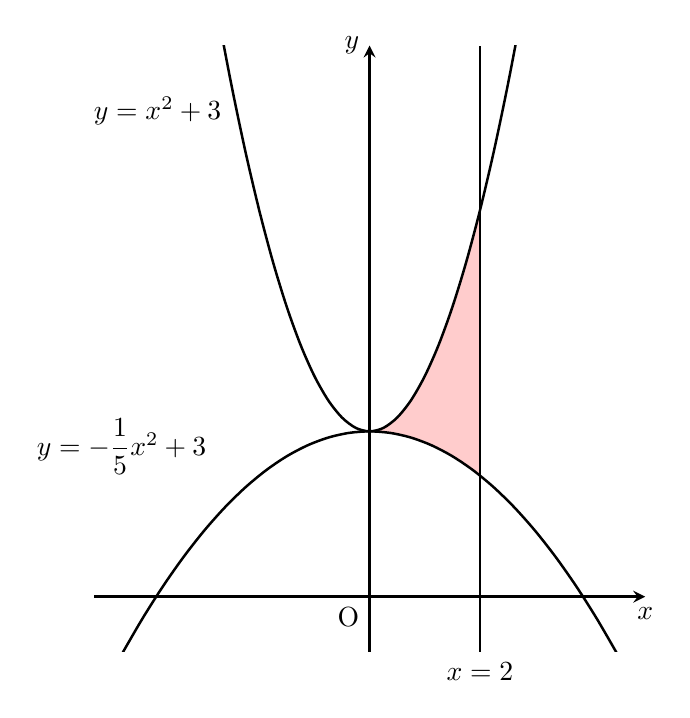
\begin{tikzpicture}[scale=.7,declare function={f(\t)=(\t)^2 + 3; g(\t)=-(1/5)*(\t)^2 + 3;}]
  \fill[red!20] plot[domain=0:2,smooth,variable=\x] ({\x},{g(\x)}) -- (2,{f(2)}) -- plot[domain=2:0,smooth,variable=\x] ({\x},{f(\x)}) -- cycle;

  \draw[-stealth] (-5,0) -- (5,0) node[below] {$x$};
  \draw[-stealth] (0,-1) -- (0,10) node[left] {$y$};

  \begin{scope}
    \clip (-4.5,-1) rectangle (4.5,10);

    \draw[domain=-3:3,smooth,variable=\x] plot ({\x},{f(\x)});
    \draw[domain=-4.5:4.5,smooth,variable=\x] plot ({\x},{g(\x)});
  \end{scope}

  \draw (2,-1) node[below]{$x=2$} -- (2,10);

  \node[below left] at(0,0) {$\mathrm{O}$};
  \node[below left] at(-2.5,{f(-2.5)}) {$y=x^2 + 3$};
  \node[above,yshift=2mm] at(-4.5,{g(-2.5)}) {$y=-\dfrac{1}{5}x^2 + 3$};
\end{tikzpicture}

\end{document}

